\chapter{Internship context}\label{ch:context}

This chapter introduces the host company, the team I worked in, the technical ecosystem underpinning the projects, and the working method. It provides the background needed to understand the following chapters.

\section{The company: Qonto}

Qonto is a European neobank for freelancers, very small businesses and SMEs. Founded in 2017 by Alexandre Prot and Steve Anavi, it is operated by the company Olinda~SAS and offers a business account together with financial-management services: payment cards, transfers, invoicing, pre-accounting and steering tools~\cite{qonto-wiki,qonto-press}. At the time of the internship, Qonto reports on the order of 600{,}000 customers and operates in eight European countries: France, Germany, Italy, Spain, Austria, Belgium, the Netherlands and Portugal, following an expansion into four new markets in 2024~\cite{qonto-press}.

On the regulatory side, Qonto operates as a \emph{payment institution} (Payment Service Provider, PSP). This status is not a mere legal detail: it entails regulatory-reporting obligations, including the European CESOP filing addressed in Chapter~\ref{ch:cesop} and demands a high level of rigour on data reliability and traceability. The opening of a Dutch IBAN in late 2025 is precisely what made Qonto liable for the CESOP filing in the Netherlands.

\begin{figure}[H]
\centering

\includegraphics[width=0.6\textwidth]{imgs/qonto.png}
\caption{Qonto logo}
\label{fig:qonto-way-card}
\end{figure}

\section{The Data Platform team and the Qonto Way}

I completed my internship within the \emph{Data Platform} team, part of the Data department. Its mission is to provide business and other technical teams with a reliable platform for ingesting, transforming and delivering data. It owns the ``plumbing'': moving data from dozens of sources into the warehouse, guaranteeing its freshness and accuracy, and exposing the results.

Each initiative is run as a Notion \emph{project card} following the \emph{Qonto Way}, a structured lifecycle in three phases (Figure~\ref{fig:qonto-way-card}). \textbf{Value Analysis} (VA) frames the problem: an \emph{Intro \& Context}, the \emph{Definition of Done}, and the \emph{Goals}. \textbf{Value Engineering} (VE) designs the solution: a \emph{Visual Spec}, the \emph{Hard Points} (the open questions or blockers to resolve before building), the \emph{Solutions}, and a \emph{Dive-in} holding the deep implementation notes. \textbf{Build} then executes the work as a task kanban (\emph{Not started} / \emph{In progress} / \emph{Done}). I followed this method for all three projects; the card in Figure~\ref{fig:qonto-way-card} is the real one for the Tableau migration (Chapter~\ref{ch:tableau}).

\begin{figure}[H]
\centering
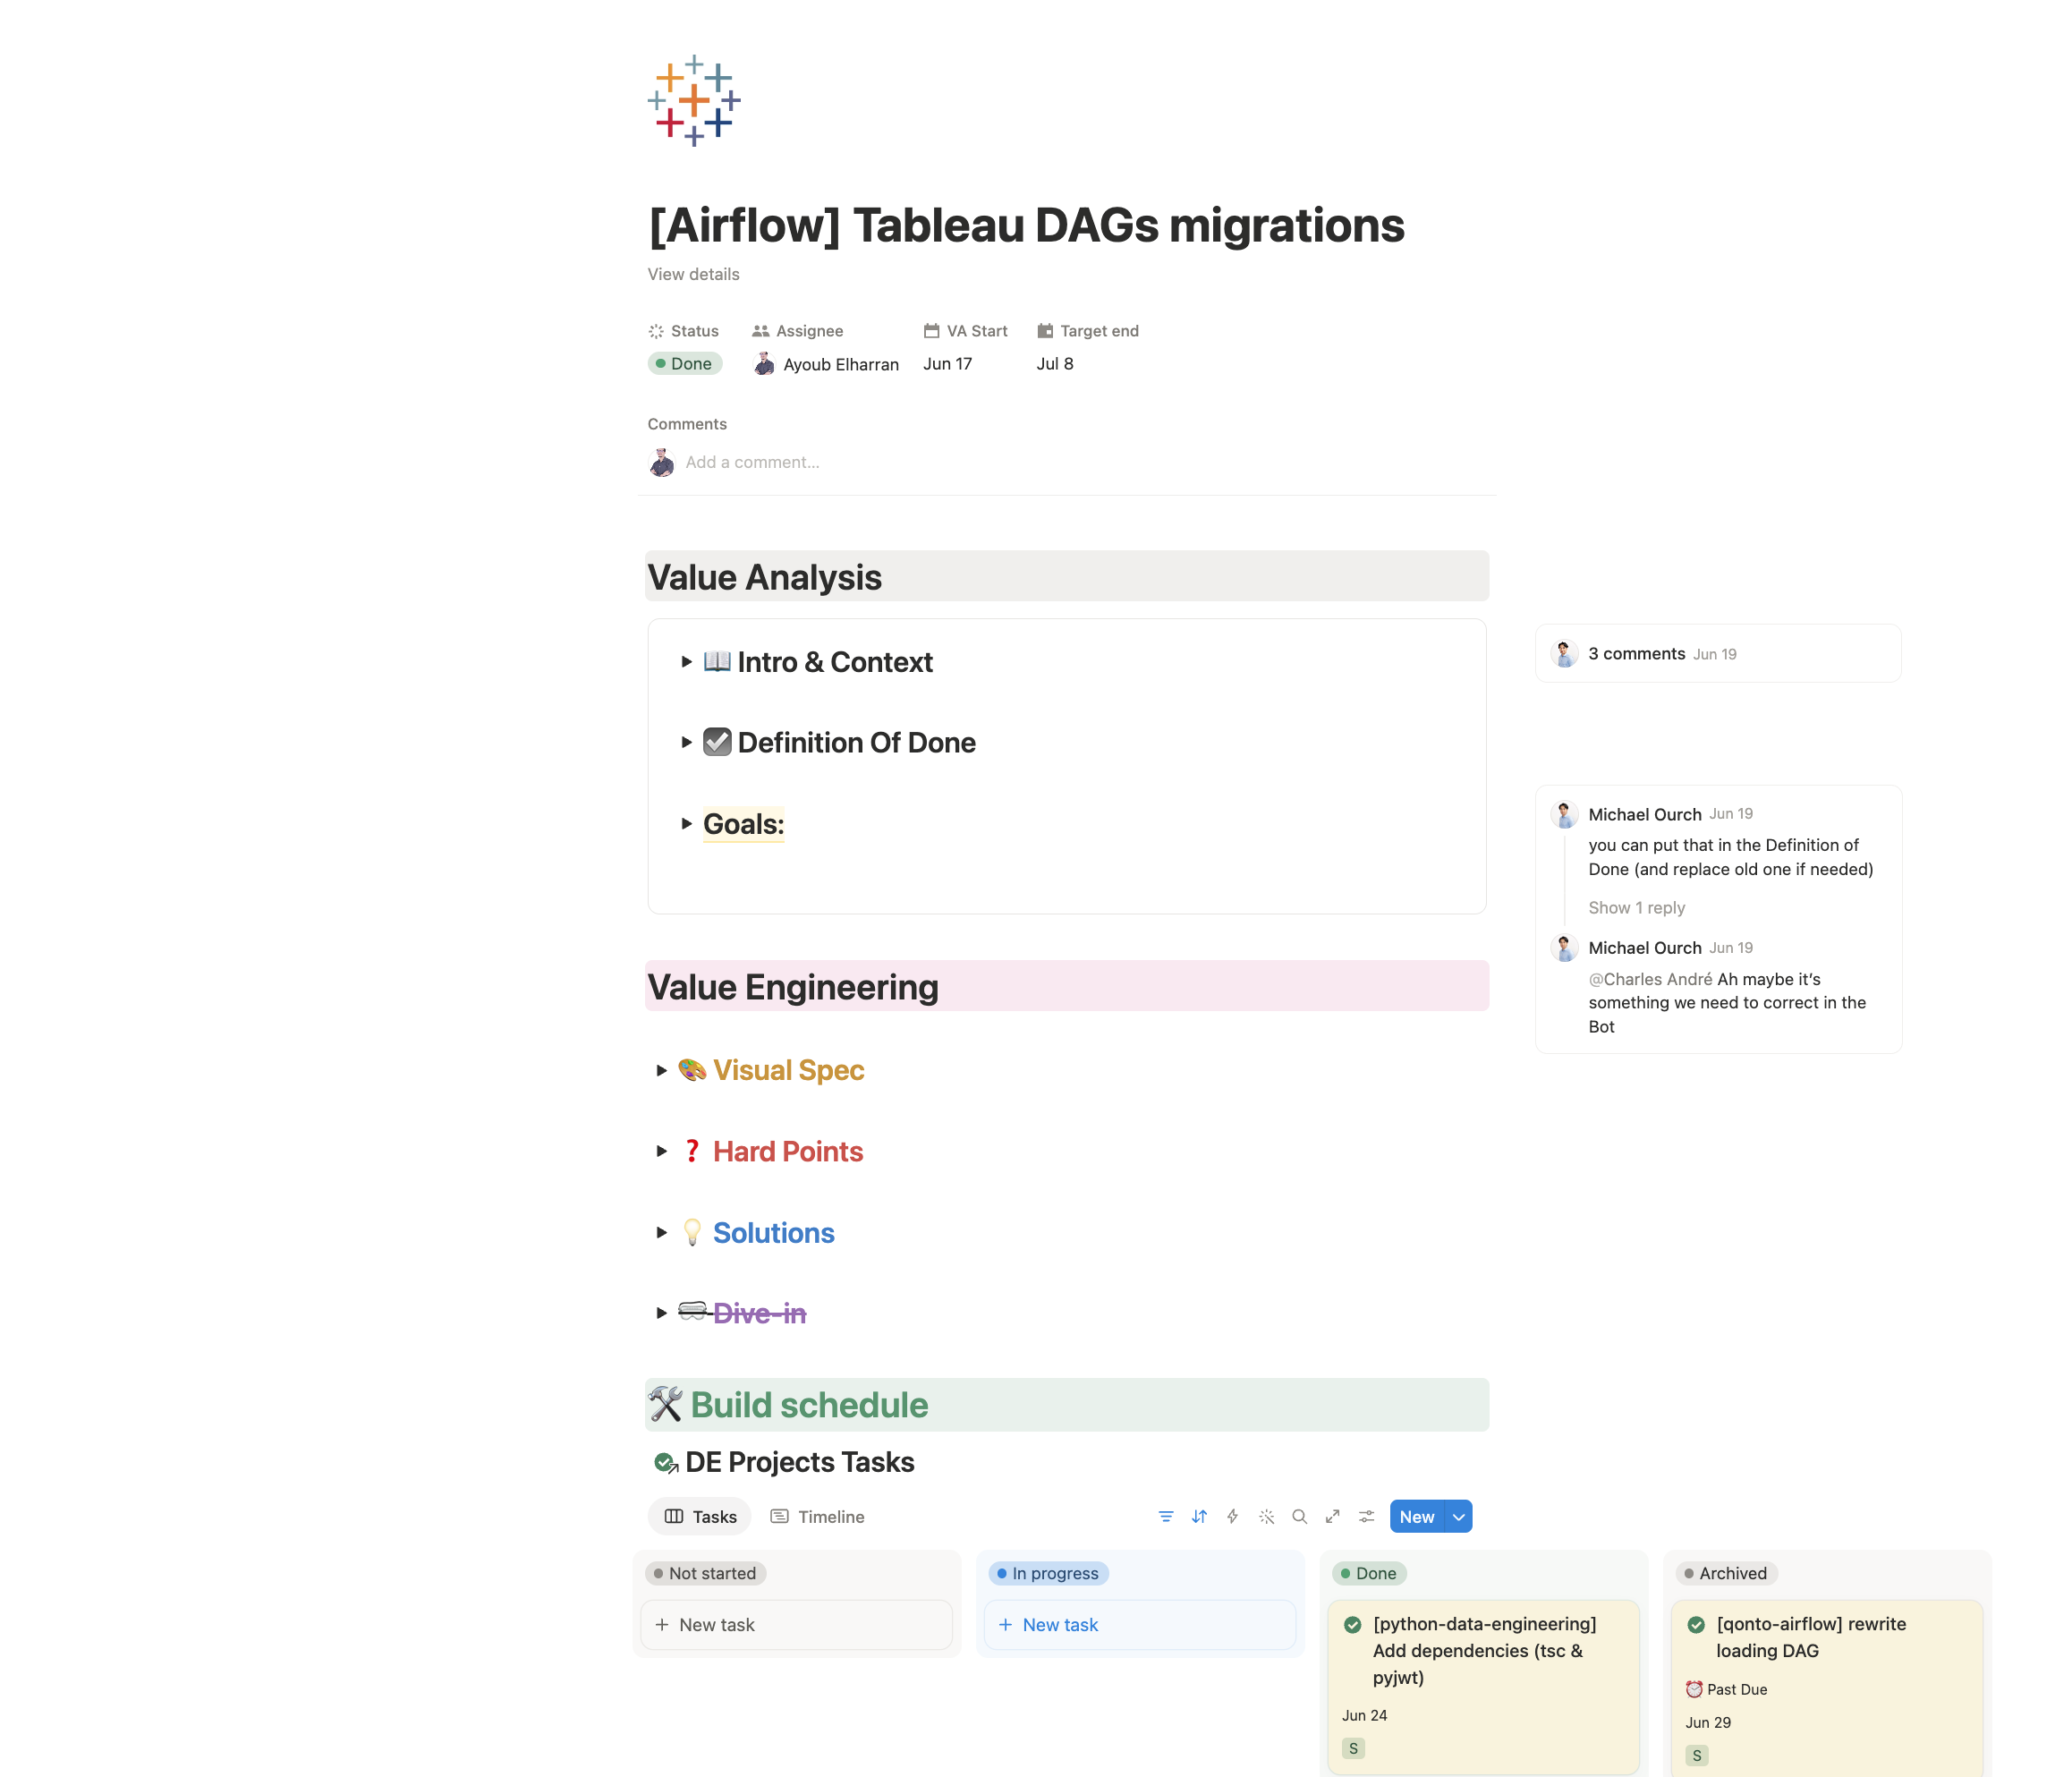
\includegraphics[width=0.8\textwidth]{imgs/project_card_page.png}
\caption{The Notion project card that structures the work following ``the Qonto Way''.}
\label{fig:qonto-way-card}
\end{figure}

At team level, a \emph{Delivery Board} tracks every project across the same lifecycle stages, \emph{Value Analysis} $\rightarrow$ \emph{Value Engineering} $\rightarrow$ \emph{Build} $\rightarrow$ \emph{Value Validation}, each with its blockers and a target date, and reviewed in a daily stand-up (Figure~\ref{fig:delivery-board}). This gave a shared, at-a-glance picture of where each initiative stood. In practice the method strongly structured my work: it forced me to pin down the \emph{Definition of Done} before coding, to surface the \emph{Hard Points} early, and to make trade-offs explicit in the \emph{Solutions} and \emph{Dive-in} sections, a discipline reflected throughout this report.

\begin{figure}[H]
\centering
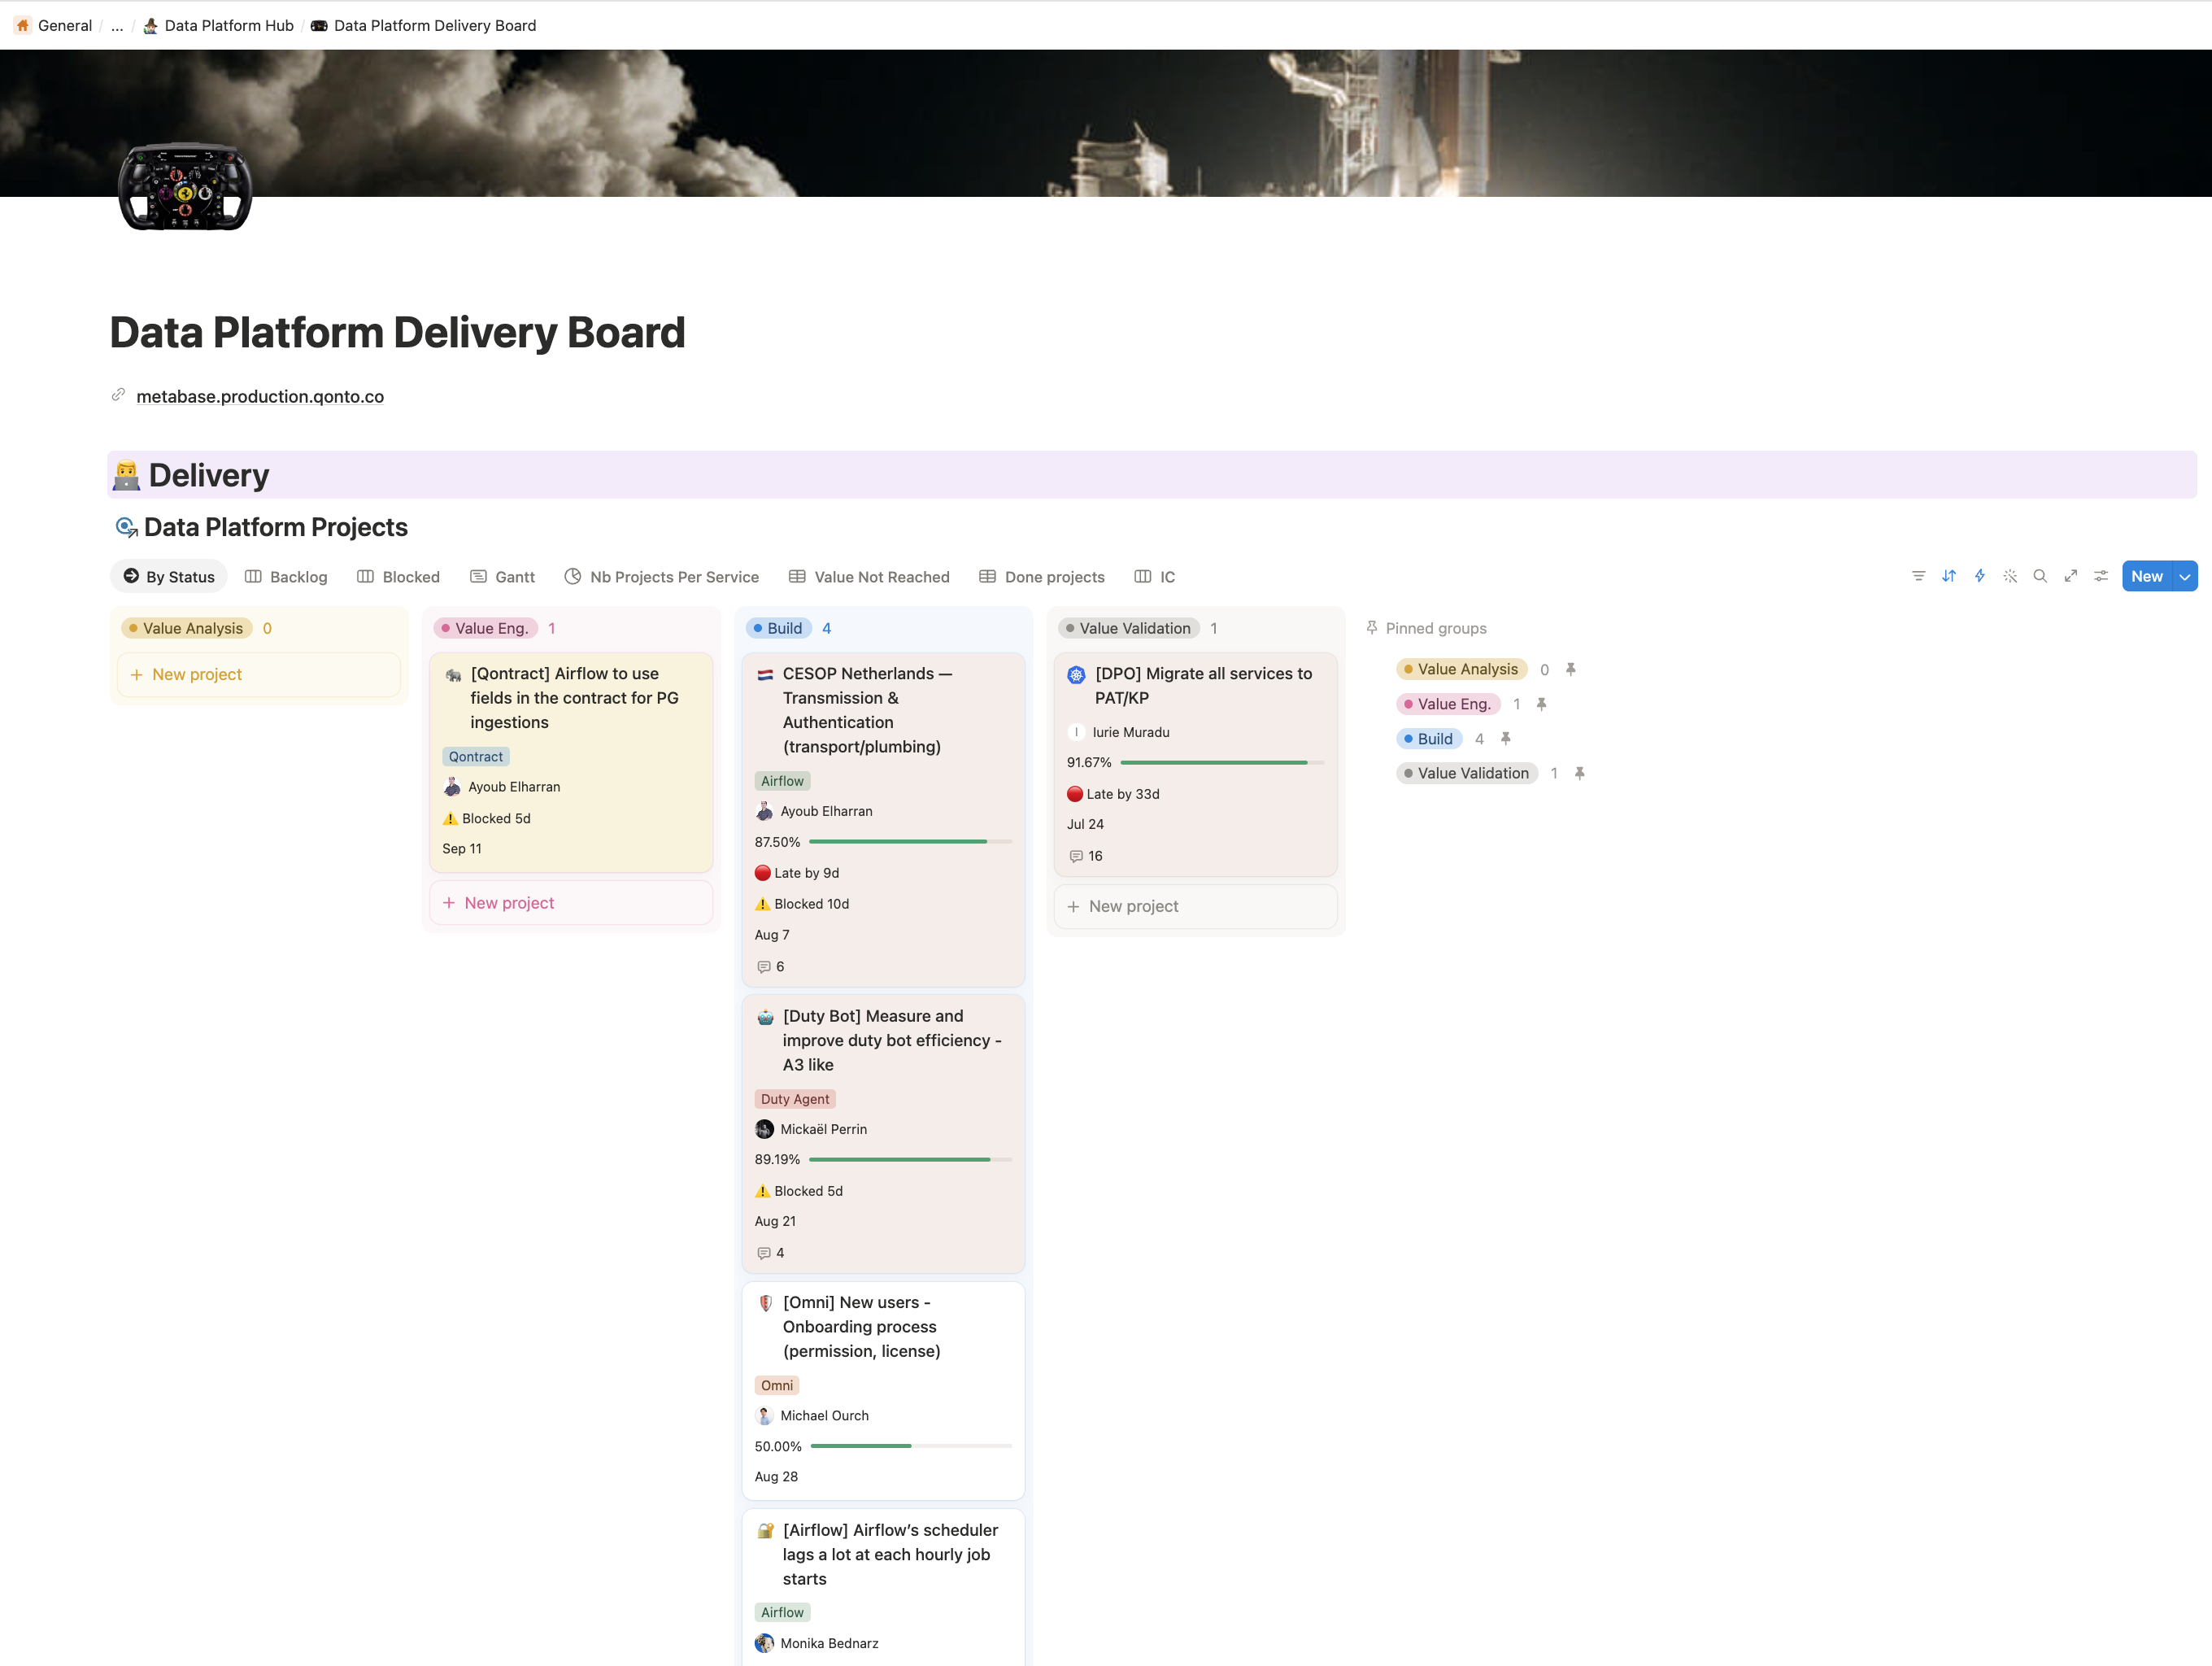
\includegraphics[width=0.8\textwidth]{imgs/data_platform_delivery_board.png}
\caption{The Data Platform Delivery Board}
\label{fig:delivery-board}
\end{figure}

On the engineering side, work goes through \emph{Pull Requests} (PRs) systematically reviewed by one or more engineers, continuous integration (tests, linting, schema validation) and a deployment across successive environments (\emph{staging} then production). This review discipline proved decisive, in particular for the zero-downtime production cutovers described later.


\section{The technical ecosystem}

The ecosystem revolves around a few building blocks (Figure~\ref{fig:archi-platform}):

\begin{itemize}
  \item \textbf{Apache Airflow} is the central orchestrator. Its code lives in a monolithic repository, \texttt{qonto-airflow}, whose distinctive feature is a \emph{declarative} generation model: rather than hand-writing each DAG, one drops a configuration file and the corresponding DAG is produced automatically. This repository relies on a \textbf{shared Docker base image} used by all pipelines; a central point for what follows.
  \begin{figure}[H]
  \centering
  
\includegraphics[width=0.2\textwidth]{imgs/airflow.png}
  \caption{Airflow logo}
  \end{figure}

  \item \textbf{Snowflake} is the cloud data warehouse, the final target of every ingestion. Raw data lands in a \texttt{RAW} database, organised by schema (one per source).
  
  \begin{figure}[H]
  \centering
  
\includegraphics[width=0.2\textwidth]{imgs/Snowflake.png}
  \caption{Snowflake logo}
  \end{figure}

  \item \textbf{Amazon S3} serves as a \emph{staging} area: extractions are written there (CSV, JSONL, Parquet) before being loaded into Snowflake with a \texttt{COPY INTO} command.
  
  \begin{figure}[H]
  \centering
  
\includegraphics[width=0.2\textwidth]{imgs/s3.png}
  \caption{Amazon S3 logo}
  \end{figure}

  \item \textbf{DBT} (\emph{data build tool}) handles downstream transformation: from the \texttt{RAW} tables, SQL models build the business tables consumed by analysts. A single DAG, \texttt{daily\_transform\_dbt}, materialises all these models with their dependencies.
  
  \begin{figure}[H]
  \centering
  \includegraphics[width=0.2\textwidth]{imgs/DBT.png}
  \caption{DBT logo}
  \end{figure}
  
  \item \textbf{Data contracts} (\emph{Qontract}) describe, as YAML files, the expected schema of each ingested table: fields, types, primary key. They are the source of truth for typing.
  \begin{figure}[H]
  \centering
  
\includegraphics[width=0.4\textwidth]{imgs/Qontract.png}
  \caption{Qontract logo}
  \end{figure}
\end{itemize}

\begin{figure}[H]
\centering
\begin{tikzpicture}[
  font=\sffamily\footnotesize,
  node distance=8mm and 12mm,
  box/.style={rectangle,rounded corners=2pt,draw=qgray!60,fill=qlight,minimum height=8mm,minimum width=20mm,align=center,inner sep=4pt},
  src/.style={box,fill=white},
  store/.style={box,fill=qaccent!12,draw=qaccent!70},
  proc/.style={box,fill=qaccent2!12,draw=qaccent2!70},
  arr/.style={-{Stealth[length=2mm]},draw=qgray,thick}
]
\node[src] (sources) {Sources\\{\scriptsize Notion, Tableau,}\\{\scriptsize APIs, Postgres\dots}};
\node[proc,right=of sources] (airflow) {Airflow\\{\scriptsize (ingestion)}};
\node[store,right=of airflow] (s3) {S3\\{\scriptsize staging}};
\node[store,right=of s3] (raw) {Snowflake\\\texttt{RAW}};
\node[proc,below=10mm of raw] (dbt) {dbt\\{\scriptsize transform}};
\node[store,left=of dbt] (marts) {Snowflake\\{\scriptsize marts}};
\node[src,left=of marts] (bi) {Delivery\\{\scriptsize Tableau, exports}};
\draw[arr] (sources) -- (airflow);
\draw[arr] (airflow) -- (s3);
\draw[arr] (s3) -- (raw);
\draw[arr] (raw) -- (dbt);
\draw[arr] (dbt) -- (marts);
\draw[arr] (marts) -- (bi);
\end{tikzpicture}
\caption{Simplified daily ETL chain of the Data Platform.}
\label{fig:archi-platform}
\end{figure}

\subsection{Airflow and config-driven DAG generation}

Airflow models each pipeline as a \emph{DAG} (Directed Acyclic Graph): a set of tasks linked by dependencies and run on a schedule. The distinctive choice in \texttt{qonto-airflow} is that these DAGs are \emph{not} hand-written but \emph{generated from configuration}. A pipeline is described by a small configuration file placed in a conventional folder; at parse time a generator \emph{discovers} every such file, validates it into a typed configuration object, and emits one DAG per file. Adding a pipeline therefore means \emph{adding a configuration}, not writing orchestration code, which is what lets the platform scale to hundreds of pipelines with little boilerplate. The flip side motivates two of my projects: because every generated DAG shares a single Docker base image, any library living in that image is coupled to \emph{all} pipelines at once, so a version bump has a \emph{blast radius} spanning the whole platform (Figure~\ref{fig:job-orch}).

\subsection{The \emph{Job Orchestrator}: moving a job out of the shared image}

One architectural element recurs in two of the three projects: the \emph{Job Orchestrator}. It is an internal pattern for running a job \emph{outside} Airflow's Docker image. The principle: the job's code lives in a dedicated repository (for example \texttt{qonto-python-data-engineering} or \texttt{qonto-python-dlt}), with its own Docker image and its own dependencies; the job is simply declared in a \texttt{schedule.yaml} file, and a component (\texttt{custom\_jobs\_orchestrator.py}) \emph{auto-generates} the corresponding Airflow DAG, each task running in an isolated Kubernetes \emph{pod}. The benefit is twofold: the job's dependencies are \emph{decoupled} from the common image, and there is no longer any DAG code to maintain in \texttt{qonto-airflow}. This mechanism is the keystone of the first two projects.

\begin{figure}[H]
\centering
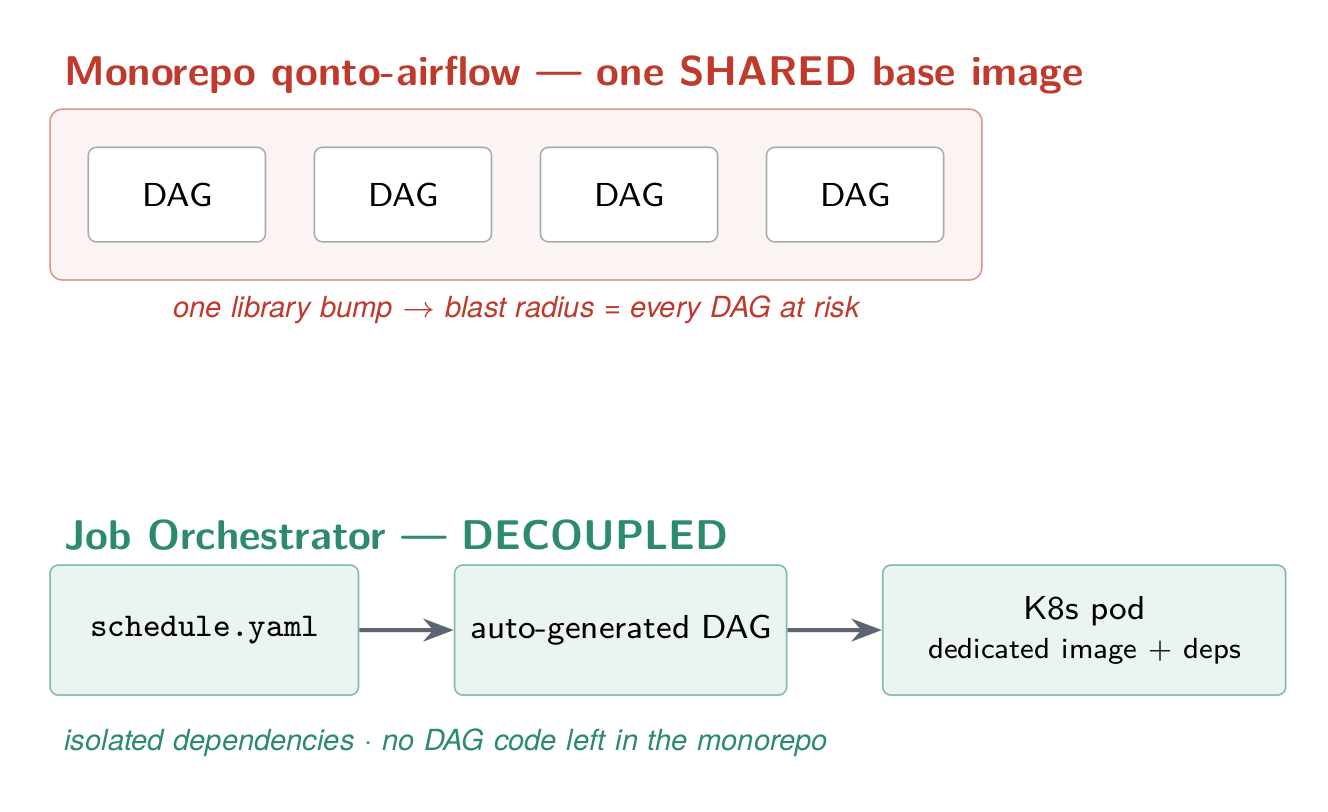
\includegraphics[width=0.8\textwidth]{imgs/job_orchestrator.png}
\caption{Airflow monorepo and the Job Orchestrator}
\label{fig:job-orch}
\end{figure}

\subsection{Data contracts: Qontract}\label{sec:qontract}

If config-driven generation is the \emph{mechanism}, \emph{Qontract} is the \emph{configuration} that sits behind every ingestion, and the reason the platform stays consistent from source to warehouse. A Qontract is a YAML \emph{data contract} (following the open ODCS~\texttt{v3.1.0} specification) that declares, for one table: its destination (Snowflake database and schema), its columns with both a \emph{logical} and a \emph{physical} type, its primary key, and an \texttt{ingestion} block telling the loader \emph{where} to read the source and \emph{how}. It is the single source of truth: the same file drives what is ingested, how each column is typed in Snowflake, and what the downstream dbt models and freshness tests expect. Listing~\ref{lst:qontract} shows a condensed real contract, the Notion \texttt{data\_bugs} board.

\begin{lstlisting}[language=yaml,caption={A contract example for the Notion data\_bugs table.},label={lst:qontract}]
apiVersion: 'v3.1.0'
kind: 'DataContract'
id: 'urn:datacontract:notion:raw:notion:data_bugs'
version: '1.0.0'
status: 'active'
servers:
  - { type: snowflake, database: raw, schema: notion }   # destination
schema:
  - name: 'data_bugs'
    logicalType: 'object'
    physicalType: 'table'
    properties:
      - { name: 'id',           logicalType: string,    physicalType: text,          primaryKey: true, required: true }
      - { name: 'Name',         logicalType: string,    physicalType: text }
      - { name: 'Status',       logicalType: string,    physicalType: text }
      - { name: 'created_time', logicalType: timestamp, physicalType: timestamp_ntz, required: true }
      - { name: 'Resolved At',  logicalType: date,      physicalType: date }
      - { name: 'archived',     logicalType: boolean,   physicalType: boolean,       required: true }
customProperties:
  - property: 'source_type'
    value: 'notion'
  - property: 'ingestion'
    value:
      page_size: 50
      resource_id: '2e7b3f6c73bc4dg49fef375e932d20e1'   # which Notion data source to read
\end{lstlisting}

Two things make the contract operational. First, the \texttt{ingestion} block is what the config-driven generator turns into a running job: \texttt{resource\_id} identifies the exact Notion data source to query and \texttt{page\_size} caps each API page. Second, the loader maps every property's declared type to a Snowflake type (Table~\ref{tab:type-map}); applying that mapping \emph{from the contract} rather than guessing it from the data is what guarantees a stable schema at every load. Chapter~\ref{ch:notion} shows the code that performs this parsing (\texttt{build\_resource\_from\_contract} and \texttt{yaml\_to\_dlt\_columns}).

\begin{table}[H]
\centering\small
\begin{tabular}{@{}lll@{}}
\toprule
\textbf{Contract} (logical / physical) & \textbf{Snowflake type} & \textbf{Example column} \\
\midrule
string / text & \texttt{TEXT} & \texttt{Name}, \texttt{Status} \\
timestamp / timestamp\_ntz & \texttt{TIMESTAMP\_NTZ} & \texttt{created\_time} \\
date / date & \texttt{DATE} & \texttt{Resolved At} \\
boolean / boolean & \texttt{BOOLEAN} & \texttt{archived} \\
number / number & \texttt{NUMBER(38,6)} & --- \\
array, object / variant & \texttt{VARIANT} & labels, people\dots \\
\bottomrule
\end{tabular}
\caption{How a Qontract property type maps to a Snowflake column type.}
\label{tab:type-map}
\end{table}

\section{My position and assignments}

Integrated into the team as a data engineer intern, I took ownership of topics end to end, from analysis to production. My three main assignments, presented in the following chapters, were: (i)~migrating Notion ingestion to the dlt framework; (ii)~migrating the Tableau pipelines out of the Airflow image with a move to JWT authentication; and (iii)~building the CESOP regulatory transmission chain for the Netherlands.